\section{Counters}
As a first step towards accomplishing our research vision, let's begin with a
\emph{simple} CRDT with \emph{simple} operations and a \emph{simple} invariant
language: PN-counters and linear equations and inequalities.

\subsection{Overview}
Recall that a \emph{G-Counter} CRDT is an increment-only counter
\cite{shapiro2011comprehensive}. A state-based G-Counter distributed across $n$
machines $1, 2, \ldots, n$ can be implemented as an $n$-tuple $(x_1, x_2,
\ldots, x_n)$ of natural numbers. The \emph{increment($k$) method} at machine
$i$ increments $x_i$ by $k$; the \emph{query method} returns the sum of the
tuple $\sum_{i=1}^n x_i$; and the \emph{merge method} computes the pairwise max
of two $n$-tuples.

A \emph{PN-Counter} CRDT is a counter which supports increments and decrements
and can be implemented as a pair $(p, n)$ of two G-Counters
\cite{shapiro2011comprehensive}. increment($x$) increments $p$ by $x$;
decrement($x$) increments $n$ by $x$; query returns $p - n$; and merge performs
a pairwise merge of $p$ and $n$.

Our \emph{invariant language} is formed from \emph{linear equations} (e.g. $x =
0$, $2x = y$, $-x + 42y - 2z = 16$) and \emph{inequalities} (e.g. $x > 0$, $2x
\leq y$, $-x + 42y - 2z \neq 16$) connected with the boolean connectives
\emph{and} ($\land$), \emph{or} ($\lor$), and \emph{not} ($\lnot$) (e.g.
$\lnot((\lnot(x < 0) \lor 2x = y) \land -x + 42y - 2z \geq 16)$).

A \emph{transaction} chooses a subset of variables and decrements or increments
each by a constant amount. For example, a transaction may increment $x$ by 1,
decrement $y$ by 42, and increment $z$ by 100.

Given a set of transactions and an invariant, we want to determine whether the
transactions are \iconfluent{} with respect to the invariant. For example, the
transaction that \emph{increments} $x$ by 1 is invariant confluent with respect
to the invariant $x > 0$, but the transaction that \emph{decrements} $x$ by 1
is not, as shown in \figref{decrement}.

\begin{figure}[h]
  \centering
  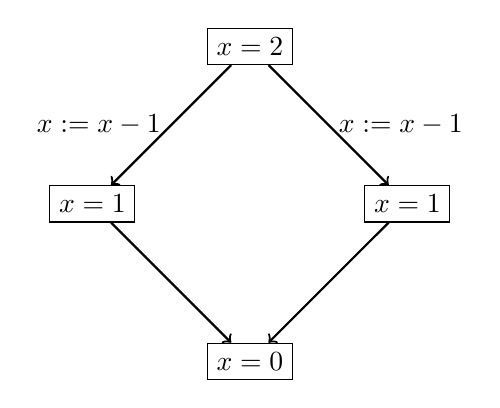
\begin{tikzpicture}
    % \draw (0, 0) grid (4, 4);
    \node[draw] (start)  at (2, 4) {$x=2$};
    \node[draw] (left)   at (0, 2) {$x=1$};
    \node[draw] (right)  at (4, 2) {$x=1$};
    \node[draw] (merged) at (2, 0) {$x=0$};

    \draw[thick, ->] (start) to node[left]  {$x := x - 1$} (left);
    \draw[thick, ->] (start) to node[right] {$x := x - 1$} (right);
    \draw[thick, ->] (left)  to (merged);
    \draw[thick, ->] (right) to (merged);
  \end{tikzpicture}
  \caption{
    A counterexample showing transaction $x := x - 1$ is not invariant
    confluent with respect to the invariant $x > 0$. The top, left, and right
    states satisfy the invariant, but the bottom state does not.
  }
  \label{fig:decrement}
\end{figure}

\subsection{Formalizing the Question}
\newcommand{\var}{\textsf{Var}}
\newcommand{\ints}{\mathbb{Z}}

Our invariant language is defined by the grammar in \figref{invariant-grammar}
which includes linear equations and inequalities over variables in a finite set
$\var$ and integer constants in $\ints$.

\begin{figure}[h]
  \centering

  \newcommand{\atom}{\textsf{atom}}
  \newcommand{\aexp}{\textsf{aexp}}
  \newcommand{\bexp}{\textsf{bexpr}}
  \begin{gather*}
    \begin{array}{rrll}
      \atom & ::= & k & \text{\emph{constants}} \\
            & |   & x & \text{\emph{variables}} \\
      &&& \\
      \aexp  & ::= & \atom         & \text{\emph{atom}} \\
             & |   & -\atom        & \text{\emph{negation}} \\
             & |   & \aexp + \aexp & \text{\emph{addition}} \\
             & |   & \aexp - \aexp & \text{\emph{subtraction}} \\
      &&& \\
      \bexp  & ::= & \aexp \leq \aexp  & \text{\emph{inequality}} \\
             & |   & \lnot \bexp       & \text{\emph{negation}} \\
             & |   & \bexp \land \bexp & \text{\emph{conjunction}} \\
             & |   & \bexp \lor \bexp  & \text{\emph{disjunction}} \\
    \end{array}
  \end{gather*}

  \caption{
    A grammar for our linear equation and linear inequality invariant language.
    Note that the comparison operators $=$, $\neq$, $<$, $>$, and $\geq$ are
    not included because they can be defined in terms of the existing
    operators.
  }
  \label{fig:invariant-grammar}
\end{figure}

A \emph{database state} is a total function $D: \var \to \ints$.  We say a
database state $D$ \emph{satisfies invariant} $I$ if $I$ evaluates to true
after all variables in $I$ have been replaced by their mapping in $D$.

A \emph{transaction} is a partial function $t: \var \rightharpoonup \ints$.
\emph{Applying a transaction} $t$ to database state $D$, denoted by $D \circ
t$, produces a new database state defined as follows:
\[
  (D \circ t)(x) \defeq \begin{cases*}
    D(x) + t(x) & $x \in \dom{}(t)$ \\
    D(x)        & otherwise
  \end{cases*}
\]

A transaction chain $C$ created from a set of transactions $T$ is a sequence of
transactions $t_1, \ldots, t_n$ where $t_j \in T$ for $1 \leq j \leq n$. Let $D
\circ C$ be syntactic sugar for $D \circ t_1 \circ \cdots \circ t_n$. We say
$C$ \emph{satisfies invariant} $I$ if for every database state $D$ and prefix
$C'$ of $C$, $D \circ C'$ satisfies invariant $I$.

A set of transactions $T$ is \iconfluent{} with respect to invariant $I$ if for
all database states $D$ and chains $C_1$ and $C_2$ created from $T$, if $D$,
$C_1$, and $C_2$ satisfy $I$, then so does $D \circ C_1 \circ C_2$.

\subsection{A Geometric Interpretation}
\newcommand{\inva}{x + y \geq 0}
\newcommand{\invb}{x - y \geq 0}
\newcommand{\invc}{x \geq 1}
\newcommand{\invd}{x \geq 3}
\newcommand{\inv}{(\inva \land \invb \land \invc) \lor (\invd)}

Sometimes, we can eyeball whether a transaction is \iconfluent{} with respect
to an invariant. Other times, not so much. For example, which transactions are
invariant confluent with respect to the invariant $\inv$? It's not immediately
clear.  Surprisingly, we can interpret the question ``Is $T$ \iconfluent{} with
respect to $I$?'' geometrically, and doing so will make answering the question
much easier!

Consider an invariant $I$ over $n$ variables $x_1, \ldots, x_n$. If we imagine
the values of the $n$ variables as an $n$-dimensional point, then we can draw
the set of points in $\ints^n$ that satisfy $I$. In fact, if we canonicalize
$I$ by eliminating negations and converting to conjunctive normal form, then
the set of points satisfying $I$ is the intersection (for $\land)$ and union
(for $\lor$) of the solutions to a set of linear equations and inequalities,
which is always straightforward to draw.  For example, the set of points
satisfying $\inv$ is shown in \figref{geometric-example}.

\begin{figure}
  \newenvironment{griddedpic}{
    \begin{tikzpicture}
      \clip (-4, -1) rectangle (4, 4);
  }{
      \draw (-4, -1) grid (4, 4);
      \draw[ultra thick] (-4, 0) -- (4, 0);
      \draw[ultra thick] (0, -1) -- (0, 4);
    \end{tikzpicture}
  }

  \begin{subfigure}[c]{0.5\textwidth}
    \begin{griddedpic}
      \fill[red, opacity=0.4]
        (-10, 10) -- (10, -10) -- (10, 10) -- cycle;
    \end{griddedpic}
    \caption{$\inva$}
  \end{subfigure}
  \begin{subfigure}[c]{0.5\textwidth}
    \begin{griddedpic}
      \fill[blue, opacity=0.4]
        (-10, -10) -- (10, 10) -- (-10, 10) -- cycle;
    \end{griddedpic}
    \caption{$\invb$}
  \end{subfigure}

  \vspace{0.5cm}

  \begin{subfigure}[c]{0.5\textwidth}
    \begin{griddedpic}
      \fill[green, opacity=0.4]
        (-10, 1) -- (10, 1) -- (10, 10) -- (-10, 10) -- cycle;
    \end{griddedpic}
    \caption{$\invc$}
  \end{subfigure}
  \begin{subfigure}[c]{0.5\textwidth}
    \begin{griddedpic}
      \fill[orange, opacity=0.4]
        (-10, 3) -- (10, 3) -- (10, 10) -- (-10, 10) -- cycle;
    \end{griddedpic}
  \caption{$\invd$}
  \end{subfigure}

  \vspace{0.5cm}

  \begin{subfigure}[c]{\textwidth}
    \centering
    \begin{griddedpic}
      \fill[purple, opacity=0.4]
        (-1, 1) -- (-3, 3) -- (-10, 3) -- (-10, 10) -- (10, 10) -- (10, 3) --
        (3, 3) -- (1, 1) -- cycle;
    \end{griddedpic}
    \caption{$\inv$}
  \end{subfigure}

  \caption{An illustration of the solution to $\inv$.}
  \label{fig:geometric-example}
\end{figure}

Next, we can imagine a transaction $t$ as an $n$-dimensional vector $(k_{x_1},
\ldots, k_{x_n})$ where $t$ adds constant $k_{x_i}$ to variable $x_i$. Now, the
question of whether a set of transactions $T$ is \iconfluent{} with respect to
invariant $I$ has been reduced to the following question. Starting at an
arbitrary point $D$ in the solution space of $I$, if we can add vectors $t^1_1,
t^1_2, \ldots, t^1_m$ to $D$ and vectors $t^2_1, t^2_2, \ldots, t^2_n$ to $D$
all while staying in the solution space of $I$, then are we guaranteed that $D
+ t^1_1 + t^1_2 + \ldots + t^1_m + t^2_1 + t^2_2 + \ldots + t^2_n$ is in the
solution space of $I$?

Turning again to our example in \figref{geometric-example}, it is now clear
that any transaction $(k_x, k_y)$ where $y \geq 0$ and $|x| \leq y$ is
\iconfluent{} with respect to $\inv$. These are the vectors that point up and
not too far left or right.
